%%%%%%%%%%%%%%%%%%%%%%%%%%%%%%%%%%%%%%%%%%%%%%%%%%%%%%%%%%%%%%%%%%%%%%
% How to use writeLaTeX: 
%
% You edit the source code here on the left, and the preview on the
% right shows you the result within a few seconds.
%
% Bookmark this page and share the URL with your co-authors. They can
% edit at the same time!
%
% You can upload figures, bibliographies, custom classes and
% styles using the files menu.
%
% If you're new to LaTeX, the wikibook is a great place to start:
% http://en.wikibooks.org/wiki/LaTeX
%
%%%%%%%%%%%%%%%%%%%%%%%%%%%%%%%%%%%%%%%%%%%%%%%%%%%%%%%%%%%%%%%%%%%%%%
\documentclass{tufte-book}

\hypersetup{colorlinks}% uncomment this line if you prefer colored hyperlinks (e.g., for onscreen viewing)

%%
% Book metadata
%\title{A Tufte-Style Book\thanks{Thanks to Edward R.~Tufte for his inspiration.}}
\author{X. L\'opez, J. M. Matxain, D. De Sancho \& I. Casademont}
%\publisher{Publisher of This Book}
\usepackage[spanish, es-tabla]{babel}
\usepackage[utf8x]{inputenc}
\usepackage[T1]{fontenc}

\title{Qu\'imica F\'isica II - \\Pr\'acticas \\ de Ordenador}
%%
% If they're installed, use Bergamo and Chantilly from www.fontsite.com.
% They're clones of Bembo and Gill Sans, respectively.
%\IfFileExists{bergamo.sty}{\usepackage[osf]{bergamo}}{}% Bembo
%\IfFileExists{chantill.sty}{\usepackage{chantill}}{}% Gill Sans

\usepackage{microtype}

%%
% Just some sample text
\usepackage{lipsum}

%%
% For nicely typeset tabular material
\usepackage{booktabs}

%%
% For graphics / images
\usepackage{graphicx}
\setkeys{Gin}{width=\linewidth,totalheight=\textheight,keepaspectratio}
\graphicspath{{graphics/}}

% The fancyvrb package lets us customize the formatting of verbatim
% environments.  We use a slightly smaller font.
\usepackage{fancyvrb}
\fvset{fontsize=\normalsize}

%%
% Prints argument within hanging parentheses (i.e., parentheses that take
% up no horizontal space).  Useful in tabular environments.
\newcommand{\hangp}[1]{\makebox[0pt][r]{(}#1\makebox[0pt][l]{)}}

%%
% Prints an asterisk that takes up no horizontal space.
% Useful in tabular environments.
\newcommand{\hangstar}{\makebox[0pt][l]{*}}

%%
% Prints a trailing space in a smart way.
\usepackage{xspace}


\setcounter{secnumdepth}{0}

% Allows for fancy math alignments
\usepackage{amsmath}
\usepackage{bm}
%\numberwithin{equation}{chapter}
%%

% Theorems
\newtheorem{theorem}{Postulado}
 
% Prints the month name (e.g., January) and the year (e.g., 2008)
\newcommand{\monthyear}{%
  \ifcase\month\or January\or February\or March\or April\or May\or June\or
  July\or August\or September\or October\or November\or
  December\fi\space\number\year
}

% Prints an epigraph and speaker in sans serif, all-caps type.
\newcommand{\openepigraph}[2]{%
  %\sffamily\fontsize{14}{16}\selectfont
  \begin{fullwidth}
  \sffamily\large
  \begin{doublespace}
  \noindent\allcaps{#1}\\% epigraph
  \noindent\allcaps{#2}% author
  \end{doublespace}
  \end{fullwidth}
}

% Inserts a blank page
\newcommand{\blankpage}{\newpage\hbox{}\thispagestyle{empty}\newpage}

\usepackage{units}

% Typesets the font size, leading, and measure in the form of 10/12x26 pc.
\newcommand{\measure}[3]{#1/#2$\times$\unit[#3]{pc}}

% Macros for typesetting the documentation
\newcommand{\hlred}[1]{\textcolor{Maroon}{#1}}% prints in red
\newcommand{\hangleft}[1]{\makebox[0pt][r]{#1}}
\newcommand{\hairsp}{\hspace{1pt}}% hair space
\newcommand{\hquad}{\hskip0.5em\relax}% half quad space
\newcommand{\TODO}{\textcolor{red}{\bf TODO!}\xspace}
\newcommand{\ie}{\textit{i.\hairsp{}e.}\xspace}
\newcommand{\eg}{\textit{e.\hairsp{}g.}\xspace}
\newcommand{\na}{\quad--}% used in tables for N/A cells
\providecommand{\XeLaTeX}{X\lower.5ex\hbox{\kern-0.15em\reflectbox{E}}\kern-0.1em\LaTeX}
\newcommand{\tXeLaTeX}{\XeLaTeX\index{XeLaTeX@\protect\XeLaTeX}}
% \index{\texttt{\textbackslash xyz}@\hangleft{\texttt{\textbackslash}}\texttt{xyz}}
\newcommand{\tuftebs}{\symbol{'134}}% a backslash in tt type in OT1/T1
\newcommand{\doccmdnoindex}[2][]{\texttt{\tuftebs#2}}% command name -- adds backslash automatically (and doesn't add cmd to the index)
\newcommand{\doccmddef}[2][]{%
  \hlred{\texttt{\tuftebs#2}}\label{cmd:#2}%
  \ifthenelse{\isempty{#1}}%
    {% add the command to the index
      \index{#2 command@\protect\hangleft{\texttt{\tuftebs}}\texttt{#2}}% command name
    }%
    {% add the command and package to the index
      \index{#2 command@\protect\hangleft{\texttt{\tuftebs}}\texttt{#2} (\texttt{#1} package)}% command name
      \index{#1 package@\texttt{#1} package}\index{packages!#1@\texttt{#1}}% package name
    }%
}% command name -- adds backslash automatically
\newcommand{\doccmd}[2][]{%
  \texttt{\tuftebs#2}%
  \ifthenelse{\isempty{#1}}%
    {% add the command to the index
      \index{#2 command@\protect\hangleft{\texttt{\tuftebs}}\texttt{#2}}% command name
    }%
    {% add the command and package to the index
      \index{#2 command@\protect\hangleft{\texttt{\tuftebs}}\texttt{#2} (\texttt{#1} package)}% command name
      \index{#1 package@\texttt{#1} package}\index{packages!#1@\texttt{#1}}% package name
    }%
}% command name -- adds backslash automatically
\newcommand{\docopt}[1]{\ensuremath{\langle}\textrm{\textit{#1}}\ensuremath{\rangle}}% optional command argument
\newcommand{\docarg}[1]{\textrm{\textit{#1}}}% (required) command argument
\newenvironment{docspec}{\begin{quotation}\ttfamily\parskip0pt\parindent0pt\ignorespaces}{\end{quotation}}% command specification environment
\newcommand{\docenv}[1]{\texttt{#1}\index{#1 environment@\texttt{#1} environment}\index{environments!#1@\texttt{#1}}}% environment name
\newcommand{\docenvdef}[1]{\hlred{\texttt{#1}}\label{env:#1}\index{#1 environment@\texttt{#1} environment}\index{environments!#1@\texttt{#1}}}% environment name
\newcommand{\docpkg}[1]{\texttt{#1}\index{#1 package@\texttt{#1} package}\index{packages!#1@\texttt{#1}}}% package name
\newcommand{\doccls}[1]{\texttt{#1}}% document class name
\newcommand{\docclsopt}[1]{\texttt{#1}\index{#1 class option@\texttt{#1} class option}\index{class options!#1@\texttt{#1}}}% document class option name
\newcommand{\docclsoptdef}[1]{\hlred{\texttt{#1}}\label{clsopt:#1}\index{#1 class option@\texttt{#1} class option}\index{class options!#1@\texttt{#1}}}% document class option name defined
\newcommand{\docmsg}[2]{\bigskip\begin{fullwidth}\noindent\ttfamily#1\end{fullwidth}\medskip\par\noindent#2}
\newcommand{\docfilehook}[2]{\texttt{#1}\index{file hooks!#2}\index{#1@\texttt{#1}}}
\newcommand{\doccounter}[1]{\texttt{#1}\index{#1 counter@\texttt{#1} counter}}

% Generates the index
\usepackage{makeidx}
\makeindex

\begin{document}

% Front matter
%\frontmatter

% r.1 blank page
%\blankpage

%% v.2 epigraphs
%\newpage\thispagestyle{empty}
%\openepigraph{%
%The public is more familiar with bad design than good design.
%It is, in effect, conditioned to prefer bad design, 
%because that is what it lives with. 
%The new becomes threatening, the old reassuring.
%}{Paul Rand%, {\itshape Design, Form, and Chaos}
%}
%\vfill
%\openepigraph{%
%A designer knows that he has achieved perfection 
%not when there is nothing left to add, 
%but when there is nothing left to take away.
%}{Antoine de Saint-Exup\'{e}ry}
%\vfill
%\openepigraph{%
%\ldots the designer of a new system must not only be the implementor and the first 
%large-scale user; the designer should also write the first user manual\ldots 
%If I had not participated fully in all these activities, 
%literally hundreds of improvements would never have been made, 
%because I would never have thought of them or perceived 
%why they were important.
%}{Donald E. Knuth}
%



% r.3 full title page
\maketitle


%% v.4 copyright page
%\newpage
%\begin{fullwidth}
%~\vfill
%\thispagestyle{empty}
%\setlength{\parindent}{0pt}
%\setlength{\parskip}{\baselineskip}
%Copyright \copyright\ \the\year\ \thanklessauthor
%
%\par\smallcaps{Published by \thanklesspublisher}
%
%\par\smallcaps{tufte-latex.googlecode.com}
%
%\par Licensed under the Apache License, Version 2.0 (the ``License''); you may not
%use this file except in compliance with the License. You may obtain a copy
%of the License at \url{http://www.apache.org/licenses/LICENSE-2.0}. Unless
%required by applicable law or agreed to in writing, software distributed
%under the License is distributed on an \smallcaps{``AS IS'' BASIS, WITHOUT
%WARRANTIES OR CONDITIONS OF ANY KIND}, either express or implied. See the
%License for the specific language governing permissions and limitations
%under the License.\index{license}
%
%\par\textit{First printing, \monthyear}
%\end{fullwidth}

% r.5 contents
%\tableofcontents
%\listoffigures
%\listoftables

%% r.7 dedication
%\cleardoublepage
%\vfill
%\begin{doublespace}
%\noindent\fontsize{18}{22}\selectfont\itshape
%\nohyphenation
%Dedicated to those who appreciate \LaTeX{} 
%and the work of \mbox{Edward R.~Tufte} 
%and \mbox{Donald E.~Knuth}.
%\end{doublespace}
%\vfill
%\vfill


\chapter[introduccion]{Introducción general}
En este primer capítulo explicaremos los objetivos que queremos
alcanzar y cuáles son las herramientas que vamos a utilizar. En 
los siguientes capítulos utilizaremos a fondo estas herramientas.
Profundizaremos en la información que como químicos podemos extraer
de la \textit{Mecánica Cuántica} y en las relaciones que la computación 
permite establecer entre teoría y experimentos. En concreto el
problema en que nos vamos a centrar es la determinación del espectro
rotovibracional del monóxido de carbono. Después determinaremos
las variaciones en el espectro ultravioleta en presencia de 
diferentes disolventes.

Pero primero debemos introducir los fundamentos teóricos
y las herramientas que vamos a utilizar para alcanzar nuestros 
objetivos. Por un lado, la Mecánica Cuántica; por otro, 
la computación, que se usa hoy en día para resolver las ecuaciones 
mecanocuánticas. Éstas han sido incorporadas en un \textit{software}
de cálculo, \textit{Gaussian-03}, al que accederemos a través de 
los comandos del sistema operativo \textit{Linux}.

\section{Linux}
\subsection{Qué es Linux}
Linux es una familia de sistemas operativos (\textit{OS}) de código 
abierto organizados en torno al \textit{Linux kernel}, desarrollado
inicialmente por Linus Torvalds. La \textit{Free Software Foundation} 
usa el nombre GNU/Linux para referirse a la familia de sistemas 
operativos así como a distribuciones específicas, que incluyen el 
kernel pero además multitud de programas y librerías del proyecto
GNU. A pesar de que este sistema operativo no es el más extendido
para usuarios domésticos, domina en el ámbito de la supercomputación,
y ha sido la base para el desarrollo del Android OS.

\subsection{Comandos de Linux}
A pesar de que Linux dispone de un entorno gráfico análogo al de 
Windows o Mac OS X, la interfaz más importante entre el usuario y el 
sistema operativo en Linux es la \textit{terminal}. En la Tabla~
\ref{tb:commands} mostramos algunos de los comandos más habituales.
En nuestro trabajo utilizaremos tanto la terminal como el entorno
gráfico de Linux.

\begin{table}[h!]
\centering
	\scriptsize
	\begin{tabular}{l|l|l}
		Comando & Descripción & Opciones \\
		\hline
		& & \\
		\texttt{ls} & Lista de archivos y directorios & \texttt{-l}, \texttt{-lt}, \texttt{-ltr} \\ 
		\texttt{pwd} & Escribe el \textit{path} & \\ 
		\texttt{df} & Mostrar la cantidad de espacio libre en disco & \texttt{-h}\\ 
		\texttt{du} & Mostrar uso de disco por parte de archivos y directorios & \texttt{-h}\\
		\texttt{man command} & Mostrar manual del programa \texttt{command}  & \texttt{}\\ 
		\texttt{grep} & Seleccionar un argumento  & \texttt{}\\

		\texttt{bg} & Mandar proceso al \textit{background}  & \texttt{}\\ 
		\texttt{fg} & Traer proceso al \textit{foreground}  & \texttt{}\\ 
		\texttt{touch file\_name} & Crear archivo  & \\ 
		\texttt{rm file\_name} & Borrar archivo  & \texttt{-i, -r}\\ 
		\texttt{cat file\_name} & Mostrar archivo por pantalla & \\ 
		\texttt{more file\_name} & Mostrar gradualmente el archivo & \texttt{}\\ 
		\texttt{nano file\_name} & Mostrar el archivo con el editor \texttt{nano}  & \\ 
		\texttt{mv file1 file2} & Mover archivo  & \\ 
		\texttt{cp file1 file2} & Crear copia de \texttt{file1}  & \texttt{-r}\\ 
		\texttt{mkdir folder\_name} & Crear directorio  & \\ 
		\texttt{cd folder\_name} & Cambio de directorio \texttt{cd folder\_name}& \texttt{}\\ 
    \end{tabular}
    \caption{Comandos habituales en el sistema operativo Linux}
    \label{tb:commands}
\end{table}

\section{Introducción a la Química Cuántica}
Las propiedades de los átomos y moléculas están descritas
íntegramente por su función de onda, $\Psi$. Para obtener estas 
propiedades debemos ser capaces de resolver la ecuación 
de Schrödinger independiente del tiempo
\begin{equation}
    \hat{H}\Psi_\mathrm{Tot}=E_\mathrm{Tot}\Psi_\mathrm{Tot} 
\end{equation}
donde $\hat{H}$ es el operador \textit{hamiltoniano} y
$E_\mathrm{Tot}$ es la energía total. A su vez, el 
hamiltoniano se puede escribir como una suma de cinco términos
\begin{equation}
    \hat{H} = \hat{T}_N + \hat{V}_{NN} + \hat{T}_e + \hat{V}_{ee} +\hat{V}_{eN}
\end{equation}
Los dos primeros términos de esta suma se corresponden con la 
energía cinética nuclear ($\hat{T}_N$) y la energía potencial de
interacción entre núcleos ($\hat{V}_{NN}$). Ambos dependen de las
coordenadas de los núcleos atómicos, $\{R_\alpha\}$. Análogamente, 
los términos $\hat{T}_e $ y $\hat{V}_{ee}$ corresponden a la 
energía cinética y potencial de los electrones, respectivamente, y
dependen de las coordenadas de los electrones, $\{r_i\}$.
Finalmente, $\hat{V}_{eN}$ es el operador energía potencial
núcleo-electrón, y es función tanto de $\{R_\alpha\}$ como de 
$\{r_i\}$. Por tanto, podemos escribir la ecuación de Schrödinger
explicitamente de la siguiente manera
\begin{equation}
    \hat{H}\Psi_\mathrm{Tot}   =
    (\hat{T}_N + \hat{V}_{NN} + \hat{T}_e + \hat{V}_{ee} +\hat{V}_{eN})\Psi_\mathrm{Tot} 
    = E_\mathrm{Tot}\Psi_\mathrm{Tot}
    \label{eq:hamilt_terms}
\end{equation}
En los siguientes capítulos veremos qué valores adoptan
estos términos en caso tanto de átomos individuales
como en el caso de moléculas.

\chapter{Átomos}
\section{Método de Hartree Fock para átomos}
\subsection{Planteamiento de las ecuaciones}
En el caso de los átomos individuales, el término correspondiente
a la interacción entre núcleos en la Ecuación \ref{eq:hamilt_terms}
es igual a cero, $\hat{V}_{NN}=0$. Asimismo, podemos ignorar el
efecto del movimiento traslacional del átomo. Por tanto, la expresión
restante para el operador hamiltoniano es
\begin{equation}
    \hat{H}_e   =
    (\hat{T}_e + \hat{V}_{ee} +\hat{V}_{eN})
\end{equation}
Todos los términos de este hamiltoniano electrónico dependen 
exclusivamente de las coordenadas electrónicas. Para este 
hamiltoniano podremos encontrar una función de onda que
también es dependiente de las coordenadas electrónicas,
$\Psi_e(\{r_i\})$. El valor propio correspondiente a esta
función propia será la energía, $E_e$, de modo que la 
ecuación que debemos resolver es
\begin{equation}
    \hat{H}_e\Psi_e(\{r_i\})   =
    (\hat{T}_e + \hat{V}_{ee} +\hat{V}_{eN})\Psi_e(\{r_i\})= E_e\Psi_e(\{r_i\})
\end{equation}

\subsection{Soluciones para las ecuaciones}
Lamentablemente, estas ecuaciones tienen una solución analítica
sólo para átomos monoelectrónicos, a los que llamamos 
hidrogenoides. En los casos restantes, debemos usar métodos
aproximados. En particular, el método que utilizaremos nosotros
es el de Hartree-Fock (HF). 

En el método de Hartree-Fock, 
la función de onda para $N$ electrones, $\Psi^{HF}_e$, se
expresa como un conjunto de funciones monoelectrónicas (espín-
orbitales), para cada una de las cuales usamos la siguiente
descripción
\begin{equation}
    \chi(x)=\phi_i(r)\sigma(s)
\end{equation}
Los espín-orbitales tienen dos partes, espacial ($\phi$) y 
de espín ($\sigma$), y la parte de espín a su vez puede ser 
de dos tipos ($\alpha$ y $\beta$). Cuando tenemos espín 
$\alpha$, la función de onda
resultante es $\chi_i=\phi_i$, mientras que cuando tenemos
espín $\beta$, la función de onda es $\chi_i=\bar{\phi}_i$.
Para expresar la función de onda para dos electrones, usamos
el producto de los espín-orbitales, 
$\Psi_e^{HF}=\phi_1(1)\bar{\phi}_1(2)$.

Por otra parte, los electrones son \textit{fermiones}, por
lo que de acuerdo con el \textit{principio de exclusión de Pauli}
deben tener una función de onda antisimétrica. Con estos 
requisitos, podemos escribir nuestra función de onda como
\begin{equation}
    \psi_e^{HF}=\frac{1}{\sqrt{2}}(\phi_1(1)\bar{\phi}_1(2)-\phi_1(2)\bar{\phi}_1(1))
\end{equation}
que a su vez podemos escribir como un determinante
\begin{equation}
    \psi_e^{HF}=\frac{1}{\sqrt{2}} 
    \begin{vmatrix}
    \phi_1(1) & \bar{\phi}_1(1)\\ 
    \phi_1(2) & \bar{\phi}_1(2)
    \end{vmatrix}
\end{equation}
Quien propuso por primera vez este tipo de expresión fue
John C. Slater (en 1929), y por este motivo este tipo
de determinantes reciben su nombre. En general, podemos
escribir un determinante de Slater como
\begin{equation}
    \psi_e^{HF}=\frac{1}{\sqrt{2}} 
    \begin{vmatrix}
    \phi_1(1) & \bar{\phi}_1(1) & \phi_2(1) & \bar{\phi}_2(1)& ...& \phi_{N/2}(1) & \bar{\phi}_{N/2}(1)\\ 
    \phi_1(2) & \bar{\phi}_1(2) & \phi_2(2) & \bar{\phi}_2(2)& ...& \phi_{N/2}(2) & \bar{\phi}_{N/2}(2) \\
    \vdots & \vdots &\vdots &\vdots &\vdots &\vdots &\vdots \\
    \phi_1(N) & \bar{\phi}_1(N) & \phi_2(N) & \bar{\phi}_2(N)& ...& \phi_{N/2}(N) & \bar{\phi}_{N/2}(N)
    \end{vmatrix}
\end{equation}

\section{Input para el programa Gaussian}
Para resolver el problema que hemos descrito, usaremos
el programa Gaussian. Le daremos instrucciones al programa
usando un archivo de \textit{input} o archivo de entrada.
En este fichero decimos exactamente qué es lo que queremos
calcular. Los archivos de input tienen la extensión 
\texttt{.com} y su sintaxis es como en el siguiente ejemplo:
\begin{verbatim}
    $RunGauss
    %nproc=1
    %Chk=h2
    #ROHF / STO-3G gfinput pop=full

    Calculo del atomo de hidrogeno 
 
    0,2
    H
\end{verbatim}

Las tres primeras líneas son necesarias para el programa y 
no las vamos a modificar. La cuarta línea, se corresponde 
con nuestro método de cálculo (en este caso, \textit{restricted
open shell Hartree Fock}, \texttt{ROHF}), la base (\texttt{STO-3G}),
y el archivo de salida para la escritura de los espín-orbitales.
En la sexta línea escribimos el título del  cálculo.
Finalmente, incluimos la carga de nuestro átomo (0, al ser 
neutro) y su multiplicidad ($2s+1=2$, en el caso del hidrógeno
por tener un electrón individual con $s=1/2$), así como su símbolo
(\texttt{H}). A este archivo lo llamaremos \texttt{h\_atom.com}.

\section{Output de Gaussian}
El archivo de \textit{output} o de salida de Gaussian lleva
la extensión \texttt{.log}. Para generar este archivo, en 
primer lugar debemos ejecutar el programa, lo cual se consigue
ejecutando en la línea de comandos lo siguiente
\begin{verbatim}
    $> g03_v h_atom.com
\end{verbatim}
Al terminar de correr el programa, se genera el archivo de salida
correspondiente \texttt{h\_atom.log}. En él podemos encontrar todo
tipo de información, empezando por la energía total y la 
configuración electrónica. Pero antes debemos comprobar que
el cálculo haya terminado correctamente, en cuyo caso aparece la 
línea "\texttt{Normal termination of Gaussian 03}" en su 
última línea. Algo más arriba encontramos un resumen del
cálculo realizado.
\begin{small}
\begin{verbatim}
1\1\GINC-CLEANDER\SP\ROHF\STO-3G\H1(2)\POBMABEJ\01-Jan-2018\0\\
#ROHF / STO-3G gfinput pop=full\Calculo del atomo de hidrogeno\\0,2\H\\
Version=AM64L-G03RevD.01\State=2-A1G\HF=-0.4665819\
RMSD=0.00e+00\Thermal=0.\Dipole=0.,0.,0.\PG=0H[O(H1)]\\@
\end{verbatim}
\end{small}

Es importante notar la línea en la que se nos muestra el valor
de la energía, \texttt{HF=-0.4665819}, correspondiente
al cálculo realizado con el método y la base que hemos elegido.
Para ver la configuración electrónica, usaremos un programa 
llamado MOLDEN, que nos ayudará a la hora de analizar el output
del programa. Para ejecutarlo, sólo debemos escribir en nuestra
línea de comandos
\begin{verbatim}
    $> molden h_atom.log
\end{verbatim}
y en el menú correspondiente escogeremos "\texttt{Density-mode}".

\begin{table}[h!]
\centering
	\scriptsize
	\begin{tabular}{ll}
     \toprule
		1a.u. & =  4.35974812 x 10$^−18$ J  \\
		         &  =  27.2113957 eV \\
	             &  = 627.509541 Kcal/mol \\ 
		         & = 219474.625 cm$^−1$ \\ 
		        & = 6.57968374 x 10$^9$ MHz \\ 
		        & = 315773.213 K \\
		        & = 2625.49992 KJ/mol \\ 
    \bottomrule
    \end{tabular}
    \caption{Factores de conversión de la energía}
    \label{tb:commands}
\end{table}

\chapter{Moléculas: Introducción}

\section{Método de Hartree Fock para moléculas}
\subsection{Planteamiento de las ecuaciones}
Recordemos primero la ecuación que necesitamos utilizar:
\begin{equation}
    (\hat{T}_N + \hat{V}_{NN} + \hat{T}_e + \hat{V}_{ee} +\hat{V}_{eN})\Psi_\mathrm{tot}(\{R_\alpha,r_i\}) 
    = E_\mathrm{tot}\Psi_\mathrm{Tot}(\{R_\alpha,r_i\}) 
\end{equation}
En el caso de las moléculas, a diferencia de los atómos, 
$\hat{V}_{NN}\neq0$ porque tenemos más de un núcleo. Esto 
dificulta las cosas. Ahora se hace necesaria una nueva 
aproximación. Los núcleos, al tener la masa mucho más grande
que los electrones, se moverán más lentos. Supondremos que
mientras los electrones hacen su movimiento, los núcleos no
se mueven. Así, podemos asumir que el movimiento de los 
electrones y de los núcleos está desacoplado. Esta aproximación
se denomina aproximación de \textit{Born-Oppenheimer}, y en
un potencial creado por los electrones se moverían los núcleos
en el mismo sitio. 

Por lo tanto, ¿Cómo quedan, en este caso las ecuaciones que 
es necesario resolver? Primero, tendremos que resolver la 
ecuación de Schrödinger electrónica,
\begin{gather}
    \hat{H}_\mathrm{e}\Psi_\mathrm{e}=E_\mathrm{e}\Psi_\mathrm{e}\\ 
    (\hat{T}_\mathrm{e} + \hat{V}_\mathrm{ee} +\hat{V}_{eN})\Psi_\mathrm{e}(\{r_i\};\{R_\alpha\})
    = E_\mathrm{e}\{R_\alpha\}\Psi_\mathrm{e}(\{r_i\};\{R_\alpha\})
\end{gather}
En esta ecuación encontramos términos familiares, debido a que
también aparecían en el caso de los átomos. Pero ahora, la función
de onda electrónica y la energía electrónica dependen 
paramétricamente de las posiciones de los núcleos. Así, la energía
electrónica calculada nos introduce en la ecuación nuclear como
potencial, y la ecuación que necesitamos resolver para los núcleos
es
\begin{equation}
    (\hat{T}_\mathrm{N} + \hat{V}_\mathrm{NN} +E_\mathrm{e})\Psi_\mathrm{N}(\{R_\alpha\})
    = E_\mathrm{Tot}\Psi_\mathrm{N}(\{R_\alpha\})
\end{equation}
Así, introducimos el concepto de Superfície de Energia Potencial $V\{R_\alpha\}=(\hat{V}_\mathrm{NN}\{R_\alpha\}+E_\mathrm{e}\{R_\alpha\})$. Los núcleos se mueven según el potencial creado por los electrones y los otros núcleos.

\subsection{Soluciones para las ecuaciones}
En el caso de los átomos, solo necesitábamos  resolver la ecuación que correspondía a los electrones y conseguíamos así, la función de onda electrónica. En el caso de las moléculas, se deben resolver dos ecuaciones, la electrónica y la nuclear.

Como en el caso de los átomos, resolvemos la ecuación electrónica 
utilizado el método Hartree-Fock. La diferencia principal es que 
ahora los orbitales serán \tesxtit{orbitales moleculares} y no 
orbitales atómicos. Los orbitales moleculares son \textit{
combinaciones lineales de orbitales atómicos}, y están
deslocalizados a lo largo de la molécula, y no localizado como en
el modelo de Lewis. Por lo tanto, la función de onda electrónica
para una molécula de capa cerrada es,
\begin{equation}
    \psi_e^{HF}=\frac{1}{\sqrt{N}} 
    \begin{vmatrix}
    \phi_1(1) & \bar{\phi}_1(1) & \phi_2(1) & \bar{\phi}_2(1)& ...& \phi_{N/2}(1) & \bar{\phi}_{N/2}(1)\\ 
    \phi_1(2) & \bar{\phi}_1(2) & \phi_2(2) & \bar{\phi}_2(2)& ...& \phi_{N/2}(2) & \bar{\phi}_{N/2}(2) \\
    \phi_1(3) & \bar{\phi}_1(3) & \phi_2(3) & \bar{\phi}_2(3)& ...& \phi_{N/2}(3) & \bar{\phi}_{N/2}(3) \\
    \vdots & \vdots &\vdots &\vdots &\vdots &\vdots &\vdots \\
    \phi_1(N) & \bar{\phi}_1(N) & \phi_2(N) & \bar{\phi}_2(N)& ...& \phi_{N/2}(N) & \bar{\phi}_{N/2}(N)
    \end{vmatrix}
\end{equation}
como en el ejemplo de los átomos. Pero ahora los orbitales no son orbitales atómicos, como teníamos antes, sino orbitales moleculares. 

Al resolver la ecuación de Schrödinger, obtenemos la función de
onda del estado fundamental y la energía electrónica. Sustituimos
la energía electrónica en la ecuación de Schrödinger nuclear. 
Resuelta esta ecuación, pueden obtenerse se consiguen las
vibraciones y los modos de rotación de los núcleos. Los niveles
vibracionales y rotacionales se pueden calcular así, y a partir de 
las diferencias de energía, podemos comparar los resultados con los
espectros de microondas, infrarrojo y los espectros Raman. 
Teniendo en cuenta los resultados electrónicos y nucleares, los
espectros UV/Vis también se pueden calcular.

\section{Input del programa Gaussian para moléculas}
Como en el caso de los átomos, podemos utilizar el programa
Gaussian para hacer los cálculos de las moléculas. En este
caso resolveremos las ecuaciones discutidas en la Sección 3.1. 
El \textit{input} o fichero de entrada es parecido al fichero
utilizado en el caso de los átomos. Ahora tendremos que 
especificar la geometría de la molécula al programa. Los núcleos
están fijos en la geometría y el programa resolverá la ecuación
electrónica.

¿Cómo se especifica la geometría de una molécula? Hay dos formas
distintas. Una opción es dar las coordenadas cartesianas de la
molécula; la otra, utilizar la \textit{z-matrix}. En la z-matrix 
se utilizan coordinadas internas, y cuando las coordinadas
cartesianas son desconocidas, es la forma más adecuada para
concretar la geometría.

\subsection{Input de la molécula H$_2$}
\begin{verbatim}
    $RunGauss
    %nproc=1
    %Chk=h2
    #ROHF / STO-3G\ddot{A} gfinput pop=full
    [línea en blanco]
    Cálculo de la molécula de hidrogeno 
    [línea en blanco] 
    0,1
    H
    H 1 hh2
    [línea en blanco]
    hh2 0.75
\end{verbatim}

Ahora, la molécula de H$_2$ es un singlete, tiene todos los
electrones apareados. Por lo tanto, la multiplicidad es 1. Y después de la línea de 0,1, escribimos la z-matrix de la molécula de H$_2$. La distancia entre los dos átomos es de 0.75 {\AA}.

\section{Output del programa Gaussian}
Los resultados de Gaussian los tenemos en el fichero de
\textit{output} o fichero de salida, como en el ejemplo de los
átomos. Para generar este fichero, primero tenemos que ejecutar
el programa Gaussian:
\begin{verbatim}
    $> g03_v h_2.com
\end{verbatim}

Cuando el cálculo termina, se crea el fichero \texttt{h2.log}, 
y en este fichero aparecerá toda la información. ¿Cuál es la
información que nos interesa? En el caso del átomo de hidrogeno
buscamos la energía electrónica y la configuración electrónica.
Esta vez, buscaremos información parecida. En las secciones
siguientes veremos cómo conseguir más información, por ejemplo, 
el dipolo de la molécula, las cargas de los átomos, etc. Primero,
tenemos que ver que nuestro cálculo ha terminado bien. Así, 
tenemos que ir al final del fichero, y las últimas líneas tienen
que ser $"\texttt{Normal termination of Gaussian 03...}"$. Así
pues, el cálculo ha terminado bien. Un poco más arriba, aparecen
resumidos los resultados en un párrafo:
\begin{small}
\begin{verbatim}
1\1\GINC-CLEANDER\SP\RHF\STO-3G\H2\POBMABEJ\05-Jan-2010\0\\#rhf/STO-3G
gnput pop=full\\Calculo de la molecula de hidrogeno\\0,1\H\H,1,0.7\\
Version=AM64L-G03RevD.01\State=1-SGG\HF=-1.1161514-\RMSD=0.000e+00\
Thermal=0.\Dipole=0.,0.,0.\PG=D*H [C*(H1.H1)\\@
\end{verbatim}
\end{small}

La energía electrónica de la molécula de H$_2$, en la geometría
que hemos expresado es \texttt{HF=-1.1161514} u.a. Para ver los
orbitales moleculares, como los orbitales atómicos, utilizaremos
el programa MOLDEN. Tenemos que darnos cuenta que ahora en vez 
de orbitales atómicos se consiguen los orbitales moleculares, 
y que estos son las combinaciones lineales de los orbitales
atómicos.

\section{Superficie de Energía Potencial de las moléculas de H$_2$ y CO}
Debido a la aproximación Born-Oppenheimer, sabemos que a cada
geometría le corresponde una energía electrónica diferente. La
dependencia de la energía electrónica con las posiciones de los
núcleos aparece la \textit{Superficie de Energía Potencial}. 
En esta sección calcularemos la superficie energía potencial de la 
molécula de H$_2$ y CO. Para eso, tenemos que calcular la energía
electrónica que le corresponde para diferentes distancias C-O y
H-H, completando la tabla de la parte inferior (la tabla solo está
para CO, pero sería parecida para la molécula de hidrógeno).

\begin{table}[h!]
\centering
	\small
	\begin{tabular}{ll|ll|ll}
	\toprule
		R(C-O) & E$_e$ & R(C-O) & E$_e$ & R(C-O) & E$_e$ \\
		\hline
		0.90   &       & 1.08   &       & 1.19   &        \\
		0.95   &       & 1.09   &       & 1.20   &        \\
		0.98   &       & 1.10   &       & 1.22   &        \\
		1.00   &       & 1.11   &       & 1.24   &        \\
		1.01   &       & 1.12   &       & 1.26   &        \\
		1.02   &       & 1.13   &       & 1.28   &        \\
		1.03   &       & 1.14   &       & 1.30   &        \\
		1.04   &       & 1.15   &       & 1.40   &        \\
		1.05   &       & 1.16   &       & 1.50   &        \\
		1.06   &       & 1.17   &       & 1.60   &        \\
		1.07   &       & 1.18   &       & 1.70   &        \\
	\bottomrule	
    \end{tabular}
\end{table}

Al completar esta tabla, los resultados se pueden representar con 
el programa XMGRACE. Para hacer eso, estos resultados se tienen 
que guardar en un fichero (por ejemplo, h2$\_{geom}$.dat) y 
después ejecutar desde la línea de comando:
\begin{verbatim}
    $> xmgrace h2\_geom.dat
\end{verbatim}
Una vez hecho esto, conseguríamos un gráfico como el que se muestra en la Figura \ref{fig:sep}.
\begin{figure}[h!]
\centering
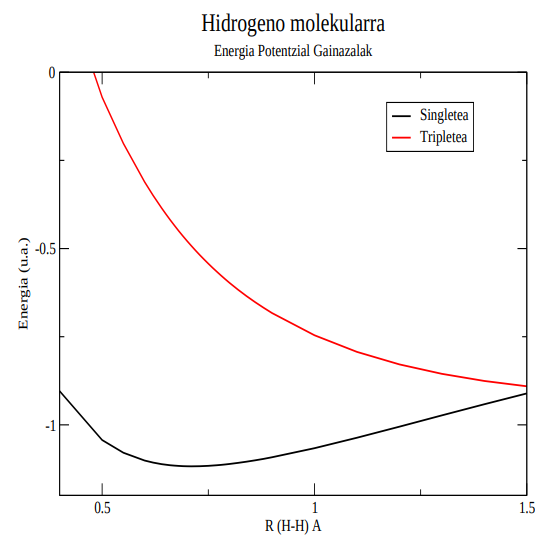
\includegraphics[scale=0.3]{PES_H2.png}
\caption{Superficie de energía potencial del hidrógeno molecular en
sus estados singlete (negro) y triplete (rojo).}
\label{fig:sep}
\end{figure}

\section{Configuración electrónica}
Los orbitales moleculares son combinaciones lineales de los
Orbitales Atómicos. En el caso del átomo de hidrógeno, tenemos el
electrón en el orbital 1s. En la molécula de H$_2$, dos orbitales
atómicos 1s se combinan para dar dos orbitales moleculares
$\sigma_g=\frac{1}{\sqrt{2}}(1s+1s)$ y 
$\sigma_u=\frac{1}{\sqrt{2}}(1s-1s)$. Con el programa Molden
podemos ver cómo se consigue el mínimo de la molécula de H$_2$ 
que  hemos observado en la figura anterior.

\chapter{Moléculas. Optimización de la geometría}
\section{Qué es la optimización de geometría? La molécula de H$_2$}
Supongamos que la geometría de la molécula que queremos 
calcular es desconocida.  En el caso de la molécula H$_2$  eso
supondría que no sabríamos la distancia de equilibrio H-H. 
La geometría óptima es aquella en la que encontramos un mínimo 
en la superficie de energía potencial. Por lo tanto, el problema
que debemos resolver es análogo al problema matemático de 
encontrar un mínimo para la función $f(x)$. En ambos casos 
podemos utilizar métodos semejantes. Uno de estos métodos es el
del gradiente conjugado. Veamos cómo funciona esta clase de 
cálculo tomado como ejemplo la molécula H$_2$.

Para realizar esta optimización debemos escribir el siguiente
texto en el archivo de input del programa Gaussian. 
\begin{verbatim}
    $RunGauss
    %nproc=1
    %Chk=h2
    #ROHF / STO-3G gfinput pop=full opt
    [línea en blanco]
    Cálculo de la molécula de hidrogeno 
    [línea en blanco] 
    0,1
    H
    H 1 hh2
    [línea en blanco]
    hh2 0.3
\end{verbatim}

¿Qué diferencia hay con los cálculos anteriores? Ahora queremos
optimizar la geometría. Para eso, tenemos que escribir 
\texttt{opt} en el input. Eso le dice a Gaussian que optimice 
la geometría. De lo contrario, haría como el primer cálculo,
calcularía la energía electrónica que corresponde a la geometría
expresada. En este caso, sabemos que la distancia H-H es 0.75 
{\AA} (ver Figura~\ref{fig:h2sing}). Para ver que la optimización
de la geometría funciona bien, podemos comenzar desde una
geometría que sabemos a ciencia cierta que es mala, por ejemplo,
0.3 {\AA} de distancia entre hidrógenos (punto 1 en la  
Fig.~\ref{fig:h2sing}). 

\begin{figure}[t!]
\centering
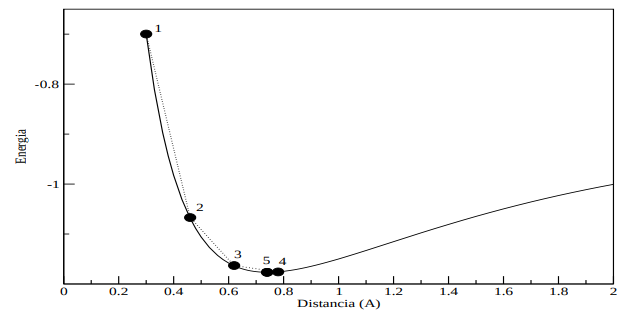
\includegraphics[scale=0.7]{PES_opt_H2.png}
\caption{Superficie de energía potencial de la molécula de H$_2$.
Los puntos corresponden a puntos sucesivos en la optimización
de la geometría.}
\label{fig:h2sing}
\end{figure}

¿Qué hace Gaussian con este input? En la Figura~\ref{fig:h2sing}
vemos cómo se va realizando la búsqueda del valor óptimo en la
superfície de energía potencial de H$_2$. En un principio, le 
hemos dicho a Gaussian que la distancia H-H es 0.3 {\AA}, y lo 
que hace  Gaussian es calcular la energía electrónica que
corresponde a esta primera distancia. Esta energía es el punto
1 del gráfico. Una 
vez hecho esto, Gaussian calcula el gradiente de la energía, y
continuado el sentido del gradiente, calcula una nueva geometría.
Con esta nueva geometría el proceso se hace otra vez. Calcula la
energía electrónica que corresponde a la nueva geometría (punto 2),
después el gradiente, y por medio del gradiente, propone una geometría nueva. Este proceso es iterativo, y termina al llegar al mínimo del Potencial, ahí mismo el gradiente es cero. Si sabemos que estamos en un mínimo (o máximo) el gradiente de esa función es cero.

En el output de Gaussian tenemos que buscar la línea que pone 
$"\texttt{Optimized parameters}"$ para buscar la geometría 
optimizada. Ahí podremos encontrar el valor resultante para 
la distancia H-H óptima, que es de 0.7122 {\AA}.

\section{Cálculo de optimización de la geometría de una molécula diatómica y de otras propiedades}
Ahora, llevaremos a cabo la optimización de la geometría 
de otras moléculas diatómicas. No solo eso. Hasta ahora no
lo hemos visto, pero Gaussian calcula muchas otras propiedades
de las moléculas y los átomos, por ejemplo, el momento dipolar,
la cargas parciales, la distribución de espín (si el espín de
la molécula no es 0). En esta sección veremos cómo conseguir 
todos estos resultados a partir de Gaussian y, completaremos 
la tabla de la parte inferior. 

Para encontrar la geometría óptima buscaremos: 
\texttt{Optimized values}. Para encontrar el momento
dipolar buscaremos: \texttt{Dipole moment}". Para encontrar 
las cargas buscaremos: \texttt{Mulliken charges}. Para 
identificar el HOMO-LUMO  \textit{gap} ($\Delta_{HL}$),
tenemos que buscar las energías asociadas a los orbitales HOMO
y LUMO. La diferencia entre  estas dos energías corresponde 
al gap HOMO-LUMO. Podemos relacionar el gap con las 
excitaciones electrónicas.

\begin{table}[h!]
\centering
	\scriptsize
	\begin{tabular}{llllll}
	\toprule
	   & R &$\mu$ & q$_1$ & q$_2$ & $\Delta_{HL}$ \\
		\hline
		H$_2$ &   &   &   &  &   \\       
		CO    &   &   &   &  &   \\       
		N$_2$ &   &   &   &  &   \\
	\bottomrule	
    \end{tabular}
\end{table}

\section{El espectro de microondas del CO}
La espectroscopia de microondas de una molécula está 
asociada con las transiciones de niveles de rotación.
En la asignatura de Química Física II hemos 
visto cuál es la interpretación física de la espectroscopía
de microondas y cómo se tiene que utilizar la Mecánica Cuántica 
para entender los espectros. Con el espectro de microondas
experimental de una molécula aprendimos a calcular las 
distancias de equilibrio, $R_e$.

Resumiendo, la diferencia entre las líneas que aparece 
en el espectro es $2B$, donde $B$ es la constante de rotación.
Utilizando la aproximación del rotor rígido, sabemos 
que la energía de los niveles de rotación es
\begin{equation}
    F(J) = BJ(J+1)
\end{equation}
siendo $J$ el número cuántico. Asimismo, la constante de 
rotación, $B$, es:
\begin{equation}
    B = \frac{\hbar}{4c\pi I}
\end{equation}
dónde $I$ es el momento de inercia de la molécula. En el 
caso de una molécula diatómica, el momento de inercia es:
\begin{equation}
    I = \mu R_e^2
\end{equation}
con la masa reducida $\mu=\frac{m_1m_2}{m_1+m_2}$.

En estas pŕacticas utilizaremos el procedimiento inverso. Al hacer
la optimización de la geometría, calculamos las distancias de
equilibrio de una molecula, $R_e$. Utilizando esto, podemos
calcular los momentos de inercia $B$ y $F(J)$, respectivamente.
Utilizando $F(J)$ y teniendo en cuenta las normas de selección
($\Delta J=\pm1$), podemos calcular el espectro de microondas.

Como ejemplo utilizaremos la molécula de HF. Teniendo en cuenta
que una molécula tiene que tener momento dipolar para tener
espectro de microondas. Para completar las tablas de la parte
inferior, primero tenemos que obtener en primer lugar el valor de
$R_e$. Los datos necesarios para hacer estos cálculos son
$\hbar=1.0545·10^{-34}$ J/s y $c=3·10^8$m/s.

\begin{table}[h!]
\centering

	\scriptsize
	\begin{tabular}{llll}
	\toprule
	    $R_e$ & $\mu$ & $I$ & $B$  \\
	\midrule	
	     &&  &  \\
	\bottomrule	
    \end{tabular}
\end{table}

\begin{table}[h!]
\centering
	\scriptsize
	\begin{tabular}{ll||ll}
	\toprule
	    Nivel Rotacional & $F (J)$ (cm $^-1$)& Transiciones & $\Delta F$ (cm$^-1$) \\
		\hline
            $J=0$  &  & $O\rightarrow1$ &   \\
            $J=1$  &  & $1\rightarrow2$ &   \\
            $J=2$  &  & $2\rightarrow3$ &   \\
            $J=3$  &  & $3\rightarrow4$ &   \\
            $J=4$  &  & $4\rightarrow5$ &   \\
            $J=5$  &  & $5\rightarrow6$ &   \\
            $J=6$  &  & $6\rightarrow7$ &   \\
            $J=7$  &  & $7\rightarrow8$ &   \\
            $J=8$  &  & $8\rightarrow9$ &   \\
            $J=9$  &  & $9\rightarrow10$&   \\
            $J=10$ &  &               &   \\
	\bottomrule	
    \end{tabular}
\end{table}


\chapter{Moléculas: Cálculo de frecuencias}

\section{Cálculo de frecuencias}
¿Qué es el cálculo de frecuencia? Al optimizar la geometría 
hemos conseguido un punto que tiene gradiente igual a cero.
Para ver si ese punto es un mínimo o un máximo se hace el 
cálculo de frecuencia. Las frecuencias están relacionadas
con la segunda derivada de la energía electrónica. Si el
gradiente en un punto en concreto es cero, podemos
determinar el valor de la segunda derivada para ver
si es un mínimo o un máximo. Si la segunda derivada es
positiva, se trata de un mínimo; si es negativa, es un
máximo.

¿Cómo llevamos a cabo este cálculo? Primero, constituimos
la matriz de las fuerzas de unión constantes. En la
diagonalización de esta matriz, se calculan los modos de
vibración normales y las frecuencias ($\tilde{\nu}_e$).

\subsection{Input de Gaussian para el cálculo de frecuencia}
Ahora vamos a ver el script de Gaussian que nos permite
realizar un cálculo de frecuencia. Como en los casos
anteriores utilizaremos la molécula de H$_2$ como ejemplo:
\begin{verbatim}
    $RunGauss
    %nproc=1
    %Chk=h2
    #RHF / STO-3G gfinput pop=full freq
    [línea en blanco]
    Cálculo de la molécula de hidrogeno 
    [línea en blanco] 
    0,1
    H
    H 1 hh2
    [línea en blanco]
    hh2 0.7122
\end{verbatim}

Comparando con el input de la optimización de la geometría,
ahora hay dos diferencias. La primera es que, ahora ya no
queremos hacer la optimización, sino el cálculo de 
frecuencias. Para eso, en vez de poner \texttt{opt} tenemos
que poner \texttt{freq}. Por otra parte, en la optimización
de la geometría, al principio no necesitábamos la distancia
exacta H-H, porque el cálculo encuentra esta distancia
óptima. Sin embargo, en el cálculo de frecuencias, la
geometría usada tiene que ser la óptima, porque esa
geometría corresponde a un mínimo de la energía electrónica.
Por eso, ahora la distancia H-H tiene que ser la distancia 
óptima que hemos calculado, 0.7122 {\AA} y no 0.3 \AA.

\subsection{Output de Gaussian del cálculo de frecuencia}
Los modos de vibración para una molécula lineal son $3N-5$, 
donde $N$ es el número de átomos.
Por lo tanto, en el caso de  las moléculas diatómicas, sólo
hay uno. Utilizando el input descrito en la sección
anterior, si ejecutamos Gaussian, el programa calculará las
frecuencias. Con el programa Molden podemos ver el modo de
vibración (cómo vibran los núcleos) y la frecuencia. 
En este caso la frecuencia es 5481.7cm$^{-1}$. Como era de
esperar, es positiva ya que corresponde a un mínimo.

\section{El espectro infrarrojo}
El espectro infrarrojo está relacionado con las frecuencias
de los modos de vibración de la molécula. ¿Cuántos modos de
vibración hay? En las moléculas lineales $3N-5$ y, en las 
no lineales $3N-6$. Los modos de vibración pueden ser de
diferentes tipos. Por una parte, los que provocan cambios 
de las distancias entre los átomos y, por otra parte, los
que provocan cambios en los ángulos. Si trabajamos en la
aproximación armónica, la frecuencia de los modos de
vibración se calcula como aparece abajo. 
\begin{equation}
    \tilde{\nu}_e = \frac{1}{2\pi c}\sqrt{\frac{k}{\mu}}
\end{equation}
donde $k$ es la constante de fuerza y siendo la segunda derivada
de la superficie de energía potencial. Una vez calculado 
$\tilde{\nu}_e$, podemos calcular los niveles de energía 
vibracional:
\begin{equation}
    G(\upsilon) = \left(\frac{1}{2}+\upsilon\right)\tilde{\nu}_e
\end{equation}
Así, podemos calcular la diferencia de energía entre
los niveles.
Y esto es el que se mide experimentalmente al hacer el espectro
infrarrojo. Por lo tanto, al calcular la frecuencia el espectro
infrarrojo se consigue directamente. En el caso de H$_2$, como
tiene el momento dipolar nulo, no tiene espectro infrarrojo. 
Con Molden, se puede ver que no aparece nada en el espectro
infrarrojo.

\section{Termoquímica}
Una vez calculadas las frecuencias, podemos conseguir las
energías vibracional, rotacional y la translacional de la 
molécula en función de la temperatura. Cuando $T=0$ K, la 
energía total de la molécula es:
\begin{equation}
    E_{Tot} = E_e+E_{vib}
\end{equation}
La energía rotacional y la traslacional son cero y todas las 
moléculas estarían en el modo vibracional fundamental. Sin
embargo, al subir la temperatura, empiezan a poblar los niveles
vibracionales superiores y además de esto, la energía rotacional
y translacional dejan de ser cero. Gaussian nos da cuál es la
energía de la molécula a temperatura ambiente, que se calcula a partir de la expresión
\begin{equation}
    E_{Tot} = E_e+E_{vib}+E_{rot}+E_{trans}
\end{equation}
Experimentalmente no se miden las diferencias de energía, sino
las diferencias de la entalpía o la energía libre de Gibbs, que se calculan como
\begin{gather}
    H = E_{Tot}+RT \\
    G = H-TS
\end{gather}
Gaussian es capaz de calcular todas estas magnitudes. Por lo
tanto, al hacer el cálculo de frecuencia, conseguimos una gran
cantidad de información:
\begin{list}{\textbullet}
\item La energía y las propiedades electrónicas (el momento
dipolar, el gap HOMO-LUMO, la carga, etc.).
\item Podemos calcular si estamos en un mínimo o un máximo 
de la Superficie de energía Potencial.
\item Calcular el espectro infrarrojo.
\item Conseguir las energías termoquímicas.
\end{list}

\chapter{Espectro rotovibracional del CO}
\section{Un poco de teoría}
En las moléculas, al contrario de lo que sucede con los 
átomos, tenemos que tener en consideración más de un 
núcleo. Por este motivo debemos hacer una primera 
aproximación, llamada de Born-Oppenheimer, de acuerdo 
con la cual desacoplamos el movimiento de electrones y 
núcleos. Por consiguiente, en primer lugar resolvemos 
la parte electrónica de la ecuación,
y usamos los valores así obtenidos a modo de potencial en la
parte nuclear de la ecuación. Para los núcleos debemos 
considerar tres tipos de movimientos: traslacional (sin
cuantizar), rotacional (cuantizado por el número cuántico $J$)
y vibracional (cuantizado en el número cuántico $v$).

Para describir el movimiento rotacional utilizamos la
aproximación del rotor rígido, con una corrección debida
a la distorsión centrífuga. Los niveles energéticos 
rotacionales resultantes son
\begin{equation}
    F(J)=B_eJ(J+1) - D_eJ^2(J+1)^2
\end{equation}
Para resolver la parte correspondiente al movimiento 
vibracional usamos la aproximación armónica con una 
corrección anarmónica,
\begin{equation}
    G(v)=\bigg(v+\frac{1}{2}\bigg)\tilde{\nu}_e - 
    \bigg(v+\frac{1}{2}\bigg)^2\chi_e\tilde{\nu}_e
\end{equation}
Estos dos movimientos, a menudo están acoplados. Cuando
el acoplamiento es pequeño podemos tratarlos de manera
independiente, pero si no es así debemos hablar de 
niveles energéticos rotovibracionales
\begin{equation}
    \begin{split}
        S(v,J)=&\bigg(v+\frac{1}{2}\bigg)\tilde{\nu}_e − 
        \bigg(v+\frac{1}{2}\bigg)^2\chi_e\tilde{\nu}_e +
        B_eJ(J+1) - \\ & DJ^2(J+1)^2 -
        \alpha_e\bigg(v+\frac{1}{2}\bigg)J(J+1)
    \end{split}
\end{equation}
En las ecuaciones anteriores usamos una serie de contantes:
$\nu_e$ es la frecuencia vibracional, $\tilde{\chi}_e$ es la
constante armónica, $B_e$ es la constante rotacional, $D$
es la constante correspondiente a la distorsión centrífuga 
y $\alpha_e$ es la constante de acoplamiento rotovibracional.

\section{Cálculo teórico de espectros}
Para simular los espectros rotovibracionales usaremos 
el programa TheoEspRotBib.py. Se trata de un programa
escriton en Python y para ejecutarlo debemos teclear
\begin{verbatim}
    $> python2.7 TheoEspRotBib.py
\end{verbatim}
El programa nos pedirá una serie de valores
\small{
\begin{verbatim}
    Molecularen izena: "CO"
    Konstante Errotazionala (cm-1): 1.9369
    Distortzio Zentrifugoa (cm-1): 0.000006
    Frequentzia Bibrazionala (cm-1): 2169.86
    anharmonizitate konstantea: 0.00612
    Akoplamendu roto-bibrazionalaren Kte (cm-1): 0.018
    Jmax-ren balioa: 30
\end{verbatim}
}
El programa generará el siguiente gráfico  
\begin{figure}
    \centering
    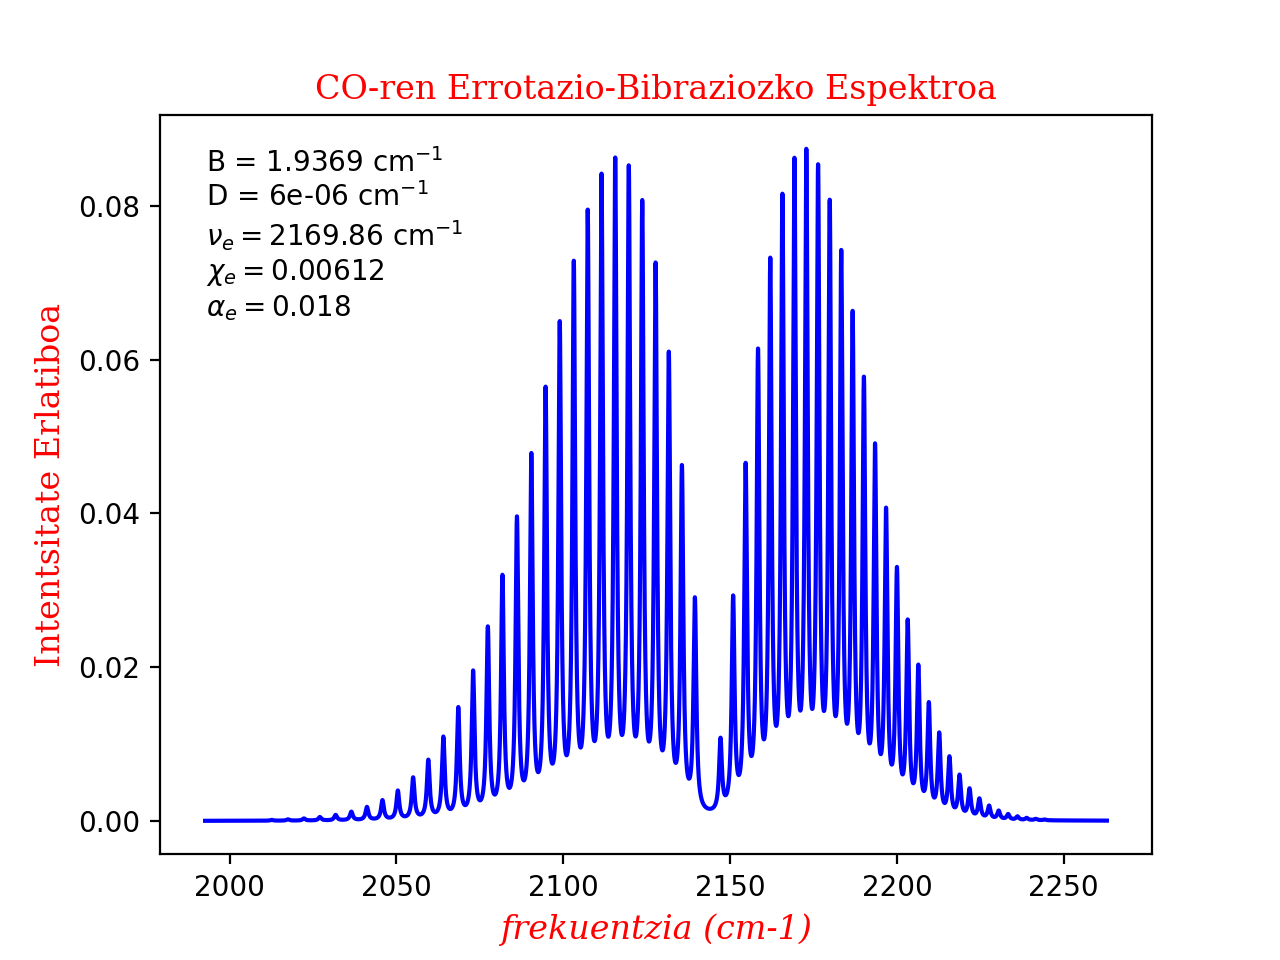
\includegraphics{figs/Figure_1.png}
    \caption{Espectro rotovibracional del monóxido de carbono.}
    \label{fig:espectro}
\end{figure}

Además, el programa generará dos ficheros: \texttt{data} y 
\texttt{data\_nuRP}. El primero de ellos contiene los datos 
del espectro, que podemos visualizar con el programa 
\texttt{xmgrace}. El archivo \texttt{data\_nuRP} permite 
comparar con las posiciones de los picos experimentales.
Data cuenta de que cada vez que se ejecuta el programa 
se generan nuevos archivos \texttt{data} y \texttt{data\_nuRP}
de tal manera que para conservar los resultados te puede 
interesar cambiar el nombre de estos archivos.

\chapter{Estados excitados del CO (espectro ultravioleta-visible)}
\section{Un poco de teoría}
Las transiciones entre niveles electrónicos son más energéticas
que las transiciones entre niveles rotovibracionales. Para que
estas transiciones sean posibles, la energía de la radiación 
incidente debe ser mayor, o lo que es lo mismo, su longitud de
onda debe ser más corta. Generalmente, en las transiciones 
electrónicas, se produce un salto de un electrón entre 
un orbital ocupado a otro no ocupado. Estas transiciones pueden
ser de diferentes tipos, dependiendo del tipo de orbital de origen 
y de destino, lo cual a su vez depende del tipo de molécula y de su
entorno.

Por ejemplo, las transiciones $\pi\rightarrow\pi^\star$ 
corresponden a la excitación de un electrón de un orbital 
$\pi$ de un enlace doble C=C para llegar a un orbital 
$\pi^\star$. En el caso de un enlace doble no conjugado,
la energía  es de 7 eV, y la radiación correspondiente
es de 180 nm (ultravioleta). En el caso de los enlaces
conjugados, la transición $\pi\rightarrow\pi^\star$
la longitud de onda es algo superior. Si un sistema
conjugado es grande, la transición puede ocurrir en
el visible. Algunos ejemoplos son la fotosíntesis y 
la isomerización. 

En esta práctica de laboratorio, y en las prácticas de 
ordenador, vamos a ver transiciones $n\rightarrow\pi^\star$,
en particular la correspondiente a la molécula de C=O
a $\sim$290 nm. Investigaremos la transición 
$n\rightarrow\pi^\star$ en acetona, y cómo cambia la 
transición cuando usamos diferentes sustituyentes o 
disolventes.

\section{Metodología}
Para calcular estas transiciones, usaremos dos métodos.
Por un lado, estimaremos el \textit{gap} HOMO-LUMO y por
otro usaremos un método más preciso denominado \textit{
Time Dependent Density Functional Theory} (TDDFT).

\section{Resultados y discusión}
\subsection{Efecto del disolvente}
Vamos a disolver la acetona en cinco disolventes diferentes
y mediremos sus transiciones electrónicas ($\lambda_{max}$).
Con los datos rellenaremos la tabla y explicaremos las
diferencias debidas a la naturaleza del disolvente.

\begin{table}[h!]
\centering
    \begin{tabular}{|l|c|c|c|c|}
    \hline
     & $\lambda_{max}$ & E(HOMO) & E(LUMO) &  $\Delta$HOMO-LUMO    \\
     \hline
    Ciclohexano &  & & &\\
    Acetonitrilo &  & & &\\
    Cloroformo  & &  & &\\
    Etanol  & & & &\\
    Agua  & & & &\\
\hline
\end{tabular}
\end{table}

\subsection{Efecto del sustituyente}
Seleccionando el ciclohexano como disolvente, vamos a probar
cinco derivados de la acetona para medir espectroscópicamente
sus transiciones electrónicas. Con los datos, rellenaremos la
siguiente tabla y explicaremos las diferencias observadas 
entre sustituyentes.

\begin{table}[h!]
\centering
    \begin{tabular}{|l|c|c|c|c|}
    \hline
     & $\lambda_{max}$ & E(HOMO) & E(LUMO) &  $\Delta$HOMO-LUMO    \\
     \hline
    Acetona &  & & &\\
    Cloruro de acetilo &  & & &\\
    Acetofenona  & &  & &\\
    Ácido acético  & & & &\\
    Metil-etil-cetona  & & & &\\
\hline
\end{tabular}
\end{table}


%\begin{thebibliography}{}
%\bibitem{atkins_depaula} Atkins, P and De Paula, J. 2006. ``Physical Chemistry, 8th Edition''. Oxford University Press.
%
%\bibitem{atkins} Atkins, P and Friedman, R. 2005. ``Molecular Quantum Mechanics, 4th Edition''. Oxford University Press.
%
%\bibitem{levine} Levine, I. N. 2013. ``Quantum
%Chemistry, 7th Edition''. Pearson.
%\end{thebibliography}

\end{document}
